% Created by tikzDevice version 0.6.1 on 2011-06-03 22:21:28
% !TEX encoding = UTF-8 Unicode
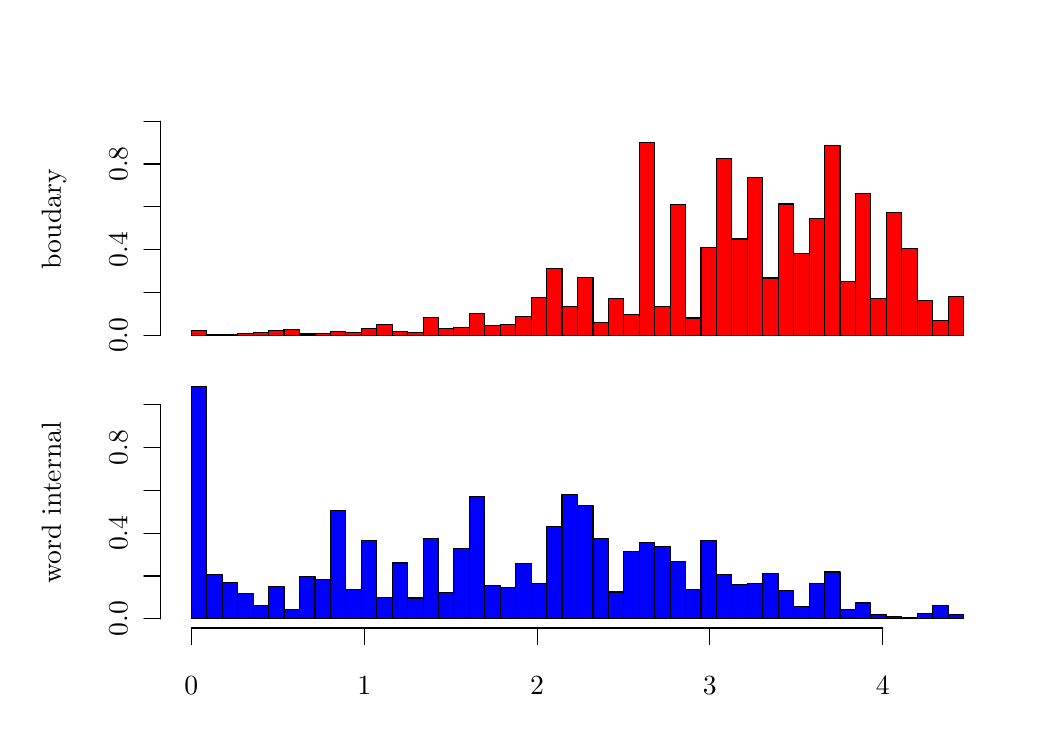
\begin{tikzpicture}[x=1pt,y=1pt]
\definecolor[named]{drawColor}{rgb}{0.00,0.00,0.00}
\definecolor[named]{fillColor}{rgb}{1.00,1.00,1.00}
\fill[color=fillColor,] (0,0) rectangle (361.35,252.94);
\begin{scope}
\path[clip] (  0.00,126.47) rectangle (361.35,252.94);
\definecolor[named]{drawColor}{rgb}{0.78,0.56,0.83}
\definecolor[named]{drawColor}{rgb}{0.00,0.00,0.00}

\node[rotate= 90.00,color=drawColor,anchor=base,inner sep=0pt, outer sep=0pt, scale=  1.00] at ( 12.00,183.71) {boudary%
};
\end{scope}
\begin{scope}
\path[clip] (  0.00,  0.00) rectangle (361.35,252.94);
\definecolor[named]{drawColor}{rgb}{0.78,0.56,0.83}
\definecolor[named]{drawColor}{rgb}{0.00,0.00,0.00}

\draw[color=drawColor,line cap=round,line join=round,fill opacity=0.00,] ( 48.00,141.82) -- ( 48.00,219.14);

\draw[color=drawColor,line cap=round,line join=round,fill opacity=0.00,] ( 48.00,141.82) -- ( 42.00,141.82);

\draw[color=drawColor,line cap=round,line join=round,fill opacity=0.00,] ( 48.00,157.29) -- ( 42.00,157.29);

\draw[color=drawColor,line cap=round,line join=round,fill opacity=0.00,] ( 48.00,172.75) -- ( 42.00,172.75);

\draw[color=drawColor,line cap=round,line join=round,fill opacity=0.00,] ( 48.00,188.22) -- ( 42.00,188.22);

\draw[color=drawColor,line cap=round,line join=round,fill opacity=0.00,] ( 48.00,203.68) -- ( 42.00,203.68);

\draw[color=drawColor,line cap=round,line join=round,fill opacity=0.00,] ( 48.00,219.14) -- ( 42.00,219.14);

\node[rotate= 90.00,color=drawColor,anchor=base,inner sep=0pt, outer sep=0pt, scale=  1.00] at ( 36.00,141.82) {0.0%
};

\node[rotate= 90.00,color=drawColor,anchor=base,inner sep=0pt, outer sep=0pt, scale=  1.00] at ( 36.00,172.75) {0.4%
};

\node[rotate= 90.00,color=drawColor,anchor=base,inner sep=0pt, outer sep=0pt, scale=  1.00] at ( 36.00,203.68) {0.8%
};
\end{scope}
\begin{scope}
\path[clip] ( 48.00,138.47) rectangle (349.35,228.94);
\definecolor[named]{drawColor}{rgb}{0.78,0.56,0.83}
\definecolor[named]{drawColor}{rgb}{0.00,0.00,0.00}
\definecolor[named]{fillColor}{rgb}{1.00,0.00,0.00}

\draw[color=drawColor,line cap=round,line join=round,fill=fillColor,] ( 59.16,141.82) rectangle ( 64.74,143.48);

\draw[color=drawColor,line cap=round,line join=round,fill=fillColor,] ( 64.74,141.82) rectangle ( 70.32,141.95);

\draw[color=drawColor,line cap=round,line join=round,fill=fillColor,] ( 70.32,141.82) rectangle ( 75.90,141.90);

\draw[color=drawColor,line cap=round,line join=round,fill=fillColor,] ( 75.90,141.82) rectangle ( 81.48,142.37);

\draw[color=drawColor,line cap=round,line join=round,fill=fillColor,] ( 81.48,141.82) rectangle ( 87.06,142.65);

\draw[color=drawColor,line cap=round,line join=round,fill=fillColor,] ( 87.06,141.82) rectangle ( 92.64,143.43);

\draw[color=drawColor,line cap=round,line join=round,fill=fillColor,] ( 92.64,141.82) rectangle ( 98.23,143.82);

\draw[color=drawColor,line cap=round,line join=round,fill=fillColor,] ( 98.23,141.82) rectangle (103.81,142.26);

\draw[color=drawColor,line cap=round,line join=round,fill=fillColor,] (103.81,141.82) rectangle (109.39,142.37);

\draw[color=drawColor,line cap=round,line join=round,fill=fillColor,] (109.39,141.82) rectangle (114.97,143.25);

\draw[color=drawColor,line cap=round,line join=round,fill=fillColor,] (114.97,141.82) rectangle (120.55,142.94);

\draw[color=drawColor,line cap=round,line join=round,fill=fillColor,] (120.55,141.82) rectangle (126.13,144.16);

\draw[color=drawColor,line cap=round,line join=round,fill=fillColor,] (126.13,141.82) rectangle (131.71,145.61);

\draw[color=drawColor,line cap=round,line join=round,fill=fillColor,] (131.71,141.82) rectangle (137.29,143.04);

\draw[color=drawColor,line cap=round,line join=round,fill=fillColor,] (137.29,141.82) rectangle (142.87,142.73);

\draw[color=drawColor,line cap=round,line join=round,fill=fillColor,] (142.87,141.82) rectangle (148.45,148.12);

\draw[color=drawColor,line cap=round,line join=round,fill=fillColor,] (148.45,141.82) rectangle (154.03,144.18);

\draw[color=drawColor,line cap=round,line join=round,fill=fillColor,] (154.03,141.82) rectangle (159.61,144.60);

\draw[color=drawColor,line cap=round,line join=round,fill=fillColor,] (159.61,141.82) rectangle (165.19,149.75);

\draw[color=drawColor,line cap=round,line join=round,fill=fillColor,] (165.19,141.82) rectangle (170.77,145.17);

\draw[color=drawColor,line cap=round,line join=round,fill=fillColor,] (170.77,141.82) rectangle (176.35,145.63);

\draw[color=drawColor,line cap=round,line join=round,fill=fillColor,] (176.35,141.82) rectangle (181.93,148.69);

\draw[color=drawColor,line cap=round,line join=round,fill=fillColor,] (181.93,141.82) rectangle (187.51,155.43);

\draw[color=drawColor,line cap=round,line join=round,fill=fillColor,] (187.51,141.82) rectangle (193.09,165.84);

\draw[color=drawColor,line cap=round,line join=round,fill=fillColor,] (193.09,141.82) rectangle (198.67,152.03);

\draw[color=drawColor,line cap=round,line join=round,fill=fillColor,] (198.67,141.82) rectangle (204.26,162.73);

\draw[color=drawColor,line cap=round,line join=round,fill=fillColor,] (204.26,141.82) rectangle (209.84,146.38);

\draw[color=drawColor,line cap=round,line join=round,fill=fillColor,] (209.84,141.82) rectangle (215.42,154.98);

\draw[color=drawColor,line cap=round,line join=round,fill=fillColor,] (215.42,141.82) rectangle (221.00,149.21);

\draw[color=drawColor,line cap=round,line join=round,fill=fillColor,] (221.00,141.82) rectangle (226.58,211.36);

\draw[color=drawColor,line cap=round,line join=round,fill=fillColor,] (226.58,141.82) rectangle (232.16,152.16);

\draw[color=drawColor,line cap=round,line join=round,fill=fillColor,] (232.16,141.82) rectangle (237.74,189.08);

\draw[color=drawColor,line cap=round,line join=round,fill=fillColor,] (237.74,141.82) rectangle (243.32,148.04);

\draw[color=drawColor,line cap=round,line join=round,fill=fillColor,] (243.32,141.82) rectangle (248.90,173.64);

\draw[color=drawColor,line cap=round,line join=round,fill=fillColor,] (248.90,141.82) rectangle (254.48,205.69);

\draw[color=drawColor,line cap=round,line join=round,fill=fillColor,] (254.48,141.82) rectangle (260.06,176.57);

\draw[color=drawColor,line cap=round,line join=round,fill=fillColor,] (260.06,141.82) rectangle (265.64,198.64);

\draw[color=drawColor,line cap=round,line join=round,fill=fillColor,] (265.64,141.82) rectangle (271.22,162.47);

\draw[color=drawColor,line cap=round,line join=round,fill=fillColor,] (271.22,141.82) rectangle (276.80,189.21);

\draw[color=drawColor,line cap=round,line join=round,fill=fillColor,] (276.80,141.82) rectangle (282.38,171.33);

\draw[color=drawColor,line cap=round,line join=round,fill=fillColor,] (282.38,141.82) rectangle (287.96,184.03);

\draw[color=drawColor,line cap=round,line join=round,fill=fillColor,] (287.96,141.82) rectangle (293.54,210.25);

\draw[color=drawColor,line cap=round,line join=round,fill=fillColor,] (293.54,141.82) rectangle (299.12,161.10);

\draw[color=drawColor,line cap=round,line join=round,fill=fillColor,] (299.12,141.82) rectangle (304.71,193.17);

\draw[color=drawColor,line cap=round,line join=round,fill=fillColor,] (304.71,141.82) rectangle (310.29,154.98);

\draw[color=drawColor,line cap=round,line join=round,fill=fillColor,] (310.29,141.82) rectangle (315.87,186.10);

\draw[color=drawColor,line cap=round,line join=round,fill=fillColor,] (315.87,141.82) rectangle (321.45,172.99);

\draw[color=drawColor,line cap=round,line join=round,fill=fillColor,] (321.45,141.82) rectangle (327.03,154.21);

\draw[color=drawColor,line cap=round,line join=round,fill=fillColor,] (327.03,141.82) rectangle (332.61,147.08);

\draw[color=drawColor,line cap=round,line join=round,fill=fillColor,] (332.61,141.82) rectangle (338.19,155.68);
\end{scope}
\begin{scope}
\path[clip] ( 48.00, 36.00) rectangle (349.35,126.47);
\definecolor[named]{drawColor}{rgb}{0.78,0.56,0.83}
\end{scope}
\begin{scope}
\path[clip] (  0.00,  0.00) rectangle (361.35,126.47);
\definecolor[named]{drawColor}{rgb}{0.78,0.56,0.83}
\definecolor[named]{drawColor}{rgb}{0.00,0.00,0.00}

\node[rotate= 90.00,color=drawColor,anchor=base,inner sep=0pt, outer sep=0pt, scale=  1.00] at ( 12.00, 81.24) {word internal%
};
\end{scope}
\begin{scope}
\path[clip] (  0.00,  0.00) rectangle (361.35,252.94);
\definecolor[named]{drawColor}{rgb}{0.78,0.56,0.83}
\definecolor[named]{drawColor}{rgb}{0.00,0.00,0.00}

\draw[color=drawColor,line cap=round,line join=round,fill opacity=0.00,] ( 59.16, 36.00) -- (308.97, 36.00);

\draw[color=drawColor,line cap=round,line join=round,fill opacity=0.00,] ( 59.16, 36.00) -- ( 59.16, 30.00);

\draw[color=drawColor,line cap=round,line join=round,fill opacity=0.00,] (121.61, 36.00) -- (121.61, 30.00);

\draw[color=drawColor,line cap=round,line join=round,fill opacity=0.00,] (184.07, 36.00) -- (184.07, 30.00);

\draw[color=drawColor,line cap=round,line join=round,fill opacity=0.00,] (246.52, 36.00) -- (246.52, 30.00);

\draw[color=drawColor,line cap=round,line join=round,fill opacity=0.00,] (308.97, 36.00) -- (308.97, 30.00);

\node[color=drawColor,anchor=base,inner sep=0pt, outer sep=0pt, scale=  1.00] at ( 59.16, 12.00) {0%
};

\node[color=drawColor,anchor=base,inner sep=0pt, outer sep=0pt, scale=  1.00] at (121.61, 12.00) {1%
};

\node[color=drawColor,anchor=base,inner sep=0pt, outer sep=0pt, scale=  1.00] at (184.07, 12.00) {2%
};

\node[color=drawColor,anchor=base,inner sep=0pt, outer sep=0pt, scale=  1.00] at (246.52, 12.00) {3%
};

\node[color=drawColor,anchor=base,inner sep=0pt, outer sep=0pt, scale=  1.00] at (308.97, 12.00) {4%
};

\draw[color=drawColor,line cap=round,line join=round,fill opacity=0.00,] ( 48.00, 39.35) -- ( 48.00,116.67);

\draw[color=drawColor,line cap=round,line join=round,fill opacity=0.00,] ( 48.00, 39.35) -- ( 42.00, 39.35);

\draw[color=drawColor,line cap=round,line join=round,fill opacity=0.00,] ( 48.00, 54.81) -- ( 42.00, 54.81);

\draw[color=drawColor,line cap=round,line join=round,fill opacity=0.00,] ( 48.00, 70.28) -- ( 42.00, 70.28);

\draw[color=drawColor,line cap=round,line join=round,fill opacity=0.00,] ( 48.00, 85.74) -- ( 42.00, 85.74);

\draw[color=drawColor,line cap=round,line join=round,fill opacity=0.00,] ( 48.00,101.21) -- ( 42.00,101.21);

\draw[color=drawColor,line cap=round,line join=round,fill opacity=0.00,] ( 48.00,116.67) -- ( 42.00,116.67);

\node[rotate= 90.00,color=drawColor,anchor=base,inner sep=0pt, outer sep=0pt, scale=  1.00] at ( 36.00, 39.35) {0.0%
};

\node[rotate= 90.00,color=drawColor,anchor=base,inner sep=0pt, outer sep=0pt, scale=  1.00] at ( 36.00, 70.28) {0.4%
};

\node[rotate= 90.00,color=drawColor,anchor=base,inner sep=0pt, outer sep=0pt, scale=  1.00] at ( 36.00,101.21) {0.8%
};
\end{scope}
\begin{scope}
\path[clip] ( 48.00, 36.00) rectangle (349.35,126.47);
\definecolor[named]{drawColor}{rgb}{0.78,0.56,0.83}
\definecolor[named]{drawColor}{rgb}{0.00,0.00,0.00}
\definecolor[named]{fillColor}{rgb}{0.00,0.00,1.00}

\draw[color=drawColor,line cap=round,line join=round,fill=fillColor,] ( 59.16, 39.35) rectangle ( 64.74,123.12);

\draw[color=drawColor,line cap=round,line join=round,fill=fillColor,] ( 64.74, 39.35) rectangle ( 70.32, 55.31);

\draw[color=drawColor,line cap=round,line join=round,fill=fillColor,] ( 70.32, 39.35) rectangle ( 75.90, 52.36);

\draw[color=drawColor,line cap=round,line join=round,fill=fillColor,] ( 75.90, 39.35) rectangle ( 81.48, 48.60);

\draw[color=drawColor,line cap=round,line join=round,fill=fillColor,] ( 81.48, 39.35) rectangle ( 87.06, 44.05);

\draw[color=drawColor,line cap=round,line join=round,fill=fillColor,] ( 87.06, 39.35) rectangle ( 92.64, 51.11);

\draw[color=drawColor,line cap=round,line join=round,fill=fillColor,] ( 92.64, 39.35) rectangle ( 98.23, 42.61);

\draw[color=drawColor,line cap=round,line join=round,fill=fillColor,] ( 98.23, 39.35) rectangle (103.81, 54.60);

\draw[color=drawColor,line cap=round,line join=round,fill=fillColor,] (103.81, 39.35) rectangle (109.39, 53.49);

\draw[color=drawColor,line cap=round,line join=round,fill=fillColor,] (109.39, 39.35) rectangle (114.97, 78.48);

\draw[color=drawColor,line cap=round,line join=round,fill=fillColor,] (114.97, 39.35) rectangle (120.55, 49.86);

\draw[color=drawColor,line cap=round,line join=round,fill=fillColor,] (120.55, 39.35) rectangle (126.13, 67.68);

\draw[color=drawColor,line cap=round,line join=round,fill=fillColor,] (126.13, 39.35) rectangle (131.71, 47.13);

\draw[color=drawColor,line cap=round,line join=round,fill=fillColor,] (131.71, 39.35) rectangle (137.29, 59.51);

\draw[color=drawColor,line cap=round,line join=round,fill=fillColor,] (137.29, 39.35) rectangle (142.87, 46.84);

\draw[color=drawColor,line cap=round,line join=round,fill=fillColor,] (142.87, 39.35) rectangle (148.45, 68.38);

\draw[color=drawColor,line cap=round,line join=round,fill=fillColor,] (148.45, 39.35) rectangle (154.03, 48.97);

\draw[color=drawColor,line cap=round,line join=round,fill=fillColor,] (154.03, 39.35) rectangle (159.61, 64.86);

\draw[color=drawColor,line cap=round,line join=round,fill=fillColor,] (159.61, 39.35) rectangle (165.19, 83.47);

\draw[color=drawColor,line cap=round,line join=round,fill=fillColor,] (165.19, 39.35) rectangle (170.77, 51.36);

\draw[color=drawColor,line cap=round,line join=round,fill=fillColor,] (170.77, 39.35) rectangle (176.35, 50.65);

\draw[color=drawColor,line cap=round,line join=round,fill=fillColor,] (176.35, 39.35) rectangle (181.93, 59.44);

\draw[color=drawColor,line cap=round,line join=round,fill=fillColor,] (181.93, 39.35) rectangle (187.51, 52.12);

\draw[color=drawColor,line cap=round,line join=round,fill=fillColor,] (187.51, 39.35) rectangle (193.09, 72.67);

\draw[color=drawColor,line cap=round,line join=round,fill=fillColor,] (193.09, 39.35) rectangle (198.67, 84.11);

\draw[color=drawColor,line cap=round,line join=round,fill=fillColor,] (198.67, 39.35) rectangle (204.26, 80.13);

\draw[color=drawColor,line cap=round,line join=round,fill=fillColor,] (204.26, 39.35) rectangle (209.84, 68.41);

\draw[color=drawColor,line cap=round,line join=round,fill=fillColor,] (209.84, 39.35) rectangle (215.42, 49.01);

\draw[color=drawColor,line cap=round,line join=round,fill=fillColor,] (215.42, 39.35) rectangle (221.00, 63.61);

\draw[color=drawColor,line cap=round,line join=round,fill=fillColor,] (221.00, 39.35) rectangle (226.58, 66.96);

\draw[color=drawColor,line cap=round,line join=round,fill=fillColor,] (226.58, 39.35) rectangle (232.16, 65.54);

\draw[color=drawColor,line cap=round,line join=round,fill=fillColor,] (232.16, 39.35) rectangle (237.74, 59.90);

\draw[color=drawColor,line cap=round,line join=round,fill=fillColor,] (237.74, 39.35) rectangle (243.32, 49.86);

\draw[color=drawColor,line cap=round,line join=round,fill=fillColor,] (243.32, 39.35) rectangle (248.90, 67.63);

\draw[color=drawColor,line cap=round,line join=round,fill=fillColor,] (248.90, 39.35) rectangle (254.48, 55.28);

\draw[color=drawColor,line cap=round,line join=round,fill=fillColor,] (254.48, 39.35) rectangle (260.06, 51.59);

\draw[color=drawColor,line cap=round,line join=round,fill=fillColor,] (260.06, 39.35) rectangle (265.64, 52.15);

\draw[color=drawColor,line cap=round,line join=round,fill=fillColor,] (265.64, 39.35) rectangle (271.22, 55.82);

\draw[color=drawColor,line cap=round,line join=round,fill=fillColor,] (271.22, 39.35) rectangle (276.80, 49.56);

\draw[color=drawColor,line cap=round,line join=round,fill=fillColor,] (276.80, 39.35) rectangle (282.38, 43.70);

\draw[color=drawColor,line cap=round,line join=round,fill=fillColor,] (282.38, 39.35) rectangle (287.96, 52.18);

\draw[color=drawColor,line cap=round,line join=round,fill=fillColor,] (287.96, 39.35) rectangle (293.54, 56.24);

\draw[color=drawColor,line cap=round,line join=round,fill=fillColor,] (293.54, 39.35) rectangle (299.12, 42.69);

\draw[color=drawColor,line cap=round,line join=round,fill=fillColor,] (299.12, 39.35) rectangle (304.71, 45.05);

\draw[color=drawColor,line cap=round,line join=round,fill=fillColor,] (304.71, 39.35) rectangle (310.29, 40.83);

\draw[color=drawColor,line cap=round,line join=round,fill=fillColor,] (310.29, 39.35) rectangle (315.87, 40.09);

\draw[color=drawColor,line cap=round,line join=round,fill=fillColor,] (315.87, 39.35) rectangle (321.45, 39.81);

\draw[color=drawColor,line cap=round,line join=round,fill=fillColor,] (321.45, 39.35) rectangle (327.03, 41.13);

\draw[color=drawColor,line cap=round,line join=round,fill=fillColor,] (327.03, 39.35) rectangle (332.61, 44.01);

\draw[color=drawColor,line cap=round,line join=round,fill=fillColor,] (332.61, 39.35) rectangle (338.19, 40.89);
\end{scope}
\end{tikzpicture}
